\documentclass[a4paper,10pt]{article}
\usepackage[margin=1cm]{geometry}
\usepackage[utf8]{inputenc}
\usepackage{hyperref}
\usepackage{url}
\usepackage{graphicx}
\usepackage{pbox}


\newcommand{\negspace}{\!\!\!}
\newcommand{\idp}{\perp \negspace \perp}
\newcommand{\nidp}{\not \idp}
\newcommand{\dep}{\top \negspace \top}
\newcommand{\ndep}{\not \dep}

%opening
\title{Uncertainty in Artificial Intelligence - Cheat sheet}
\author{Dieter Castel \& Pierre Carbonnelle}

\begin{document}

\maketitle

Original google docs by P. Carbonelle to be found here:\\ \url{https://docs.google.com/presentation/d/1sP-PJmo-pW4epfLQs3zoveZGceqw59pPeNAY9OM6dl8/edit#slide=id.p}

\section{General Probability}

$$\begin{array}{l|c}
    \textrm{ Formula} & \textrm{Comment}  \\ 
    p(x,y,z) = p(x \wedge y \wedge z) = p(x,z|y)p(y) & \textrm{Joint Probability Distribution (JPD)}\\
    \\
    p(x \vee y) = p(x) + p(y) - p(x \wedge y) & \textrm{Disjunction for probabilities} \\
    \\
    p(x|y) = \frac{p(x,y)}{p(y)} = \frac{p(y|x)p(x)}{p(y)} & \textrm{Definition of Conditional Probablity}\\
    \\
    p(\neg x) = 1-p(x) & \textrm{only valid for probability distributions i.e. normalized!} \\
    \\
    p(x) = \sum_{x,z} p(x,y,z) & \textrm{marginalisation} \\
    \\
    \sum_{y,z} p(x|y,z) = 1 & \textrm{marginalisation of CPD sums to one.} \\
    \\
    size(p(\hat{x},\hat{y},\hat{z})) = \#dom(\hat{x})*\#dom(\hat{y})*\#dom(\hat{z}) & \textrm{\textbf{without} independence assumptions} \\
    \\
    p(x_1,\ldots,x_n) = p(x_1)p(x_2|x_1)p(x_3|x_2,x_1) \ldots p(x_k|x_{k+1},\ldots,x_{n}) & Chain rule  \\ 
  \end{array}
$$

\section{Distributional Independence}

$$\begin{array}{l|c}
    \textrm{ Formula} & \textrm{Comment}  \\ 
    X \idp Y \iff  \forall x \in X, y \in Y : p(x,y) = p(x)p(y) & \textrm{marginal distributional independence for variable sets X,Y} \\
    \\
    X \idp Y \iff  \forall x \in X, y \in Y: p(x|y) = p(x) & \textrm{marginal distributional independence with CPD def.}\\
    \\
    X \idp Y | Z \iff  \forall x \in X, y \in Y : p(x|y,z) = p(x|z) & \textrm{conditional distributional independence.}\\
  \end{array}
$$

Below is the markov blanket of $x_4$: parents, childeren and parents of its childeren.
\begin{figure}[htb!]
\centering
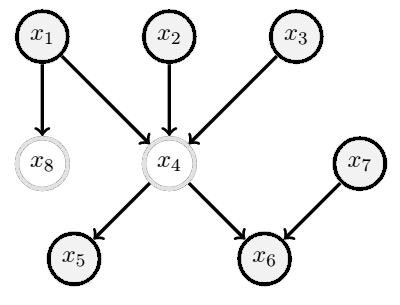
\includegraphics[scale=0.3]{gmarkovblanky.png}
\end{figure}

\newpage
\section{Graphical Independence/d-separation}
In this section $\idp$ and the like only mean GRAPHICAL independence and beware:\\
Graphical independence (== d-separation) $\Rightarrow$ distributional independence. \\
Graphical dependence (== d-connected) $\not \Rightarrow$ distributional independence. 

\begin{figure}[htb!]
\centering
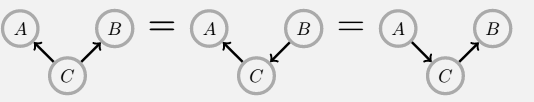
\includegraphics[scale=0.5]{gnoncollider.png}
\end{figure}
These non-colliders are equivalent from an independence point of view. 

\begin{figure}[htb!]
\begin{tabular}{l||r}
\textbf{colliders} in BN & \textbf{non-colliders} in BN \\
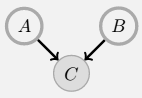
\includegraphics{gcollider.png} & 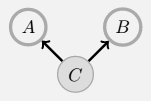
\includegraphics{gnocol.png}  \\
 \large $ A \nidp B | C$ or $ A \dep B | C$ & \large $ A \idp B | C$ or $ A \ndep B | C$ \\
\end{tabular}
\centering
\end{figure}

\subsection{Path-blocking} 
$$\forall p \in allpaths(x,y): blocked(p,Z) \rightarrow isDSeparated(x,y) $$
$$\exists p \in allpaths(x,y): infoflows(p,Z) \rightarrow isDConnected(x,y) $$

A path $p$ is $blocked(p) \iff (1) \vee (2)$
\begin{figure}[htb!]
\begin{tabular}{l||r}
 (1) COLLIDER  & NON-COLLIDER (2) \\
   & $u>v>w$ \\
  $u>v<w$  & $u<v<w$ \\
   & $u<v>w$ \\
$\exists v \in p \setminus \{x,y\} :$ &  $\exists v \in p \setminus \{x,y\} :$ \\
$collider(v) \wedge collider(v) \notin Z \wedge descendants(v) \notin Z$  &  $noncollider(v) \wedge v \in Z$
\end{tabular}
\centering
\end{figure}
(d-separation see p43 BRML.)

\subsection{AMDS on complete graph at once} 
Quickest way is with graph edits \textbf{AMDS}. For variable sets $X,Y,Z : X \idp Y | Z$
\begin{itemize}
 \item \textbf{Ancestral} graph (keep X,Y,Z and ancestors(X,Y,Z)) \begin{flushright}\textbf{A}\end{flushright}
 \item \textbf{Moralize} (add edges between all parents of the same node) ($\forall v \in A marry(parents(v))$) \begin{flushright}\textbf{M}\end{flushright}
 \item \textbf{Disorient} (remove arrows) \begin{flushright}\textbf{D}\end{flushright}
 \item \textbf{Separate} (remove all edges from nodes in Z) \begin{flushright}\textbf{S}\end{flushright}
\end{itemize}
\textbf{In the final S graph all unconnected nodes are D-separated.}

$$\begin{array}{c|c|c|c}
\textbf{symmetry} & \textbf{decomposition} & \textbf{weak union} & \textbf{contraction} \\
A \idp B | C &  A \idp B,C &  A \idp B,C & A \idp B \wedge A \idp C | B \\
\iff &  \Downarrow & \Downarrow & \Downarrow \\
B \idp A | C &  A \idp B \wedge A \idp C & A \idp B | C \wedge A \idp C | B &  A \idp B,D \\
\end{array}$$

Graphical networks are \textbf{Markov Equivalent} $\iff$ same independencies $\iff$ same skeleton $\wedge$ same immoralities.

\section{Independence Equivalencies between}

\section{General Inference}

$$\begin{array}{l|c}
    \textrm{ Formula} & \textrm{Comment}  \\ 
    p(v_{1:t}, h_{1:t}) = p(h_1) * \Pi^{t}_{i=2} p(v_t|h_t) p(h_t| h_{t-1}) & \textrm{JPD for an HMM}
    \\
    p(v_t | h_t) (= p(v_1 | h_1) \iff \textrm{stationary HMM})   & \textrm{emission matrix} \\
    \forall t p(v_t | h_t) = p(v_1 | h_1)    & \textrm{emission matrix for stationary HMM} \\
    p(h_t | h_{t-1})  & transmission matrix  \\
     & Inference in HMMS \\
    p(h_t | v_{1:t}) & Filtering (infer up to t) \ \
    p(h_t | v_{1:T}) & Smoothing (use future too) \\
    argmax_{h_1:T} p(h_{1:T} | v_{1:T}) & Viterbi (most likely state) \\
  \end{array}
$$

\section{Hidden Markov Models (HMM)}




\end{document}
